\documentclass[a4paper]{scrartcl}
\usepackage[utf8]{inputenc}
\usepackage[english]{babel}

\usepackage{amsmath}
\usepackage{amsfonts} % for mathbb for instance
\usepackage{mathtools}
\usepackage[amsmath, amsthm, framed, thmmarks]{ntheorem}

\usepackage[usenames,dvipsnames,svgnames,table]{xcolor}


% specifics about the pdf
\usepackage[english]{babel}
\usepackage[pdftex]{graphicx}
\usepackage[pdftex,bookmarks,colorlinks,pdffitwindow]{hyperref}

\usepackage{multicol}  
%\usepackage[rflt]{floatflt}  
\usepackage{epsfig} 
%\usepackage{qtree} 
\usepackage{url}

\usepackage{todonotes}

% PDF Import support
\usepackage{pdfpages}
% Support for PDF scaling
\usepackage{graphicx}
% Algorithmen
\usepackage{algorithmic}
\usepackage{algorithm}
\usepackage{listings} 
% \lstset{numbers=left, numberstyle=\tiny, numbersep=5pt} 
\lstset{
	basicstyle=\ttfamily\scriptsize\mdseries,
	keywordstyle=\bfseries\color{blue},
	identifierstyle=,
% 	stringstyle=\itshape\color{red},
	numbers=left,
	numberstyle=\tiny,
	stepnumber=10,
	breaklines=true,
	frame=none,
	showstringspaces=false,
	tabsize=4,
% 	backgroundcolor=\color{gray},
% 	morecomment=[s][\color{green}]{/+}{+/},
	commentstyle=\color{gray},	
	captionpos=b,
	float=htbp,
}
% math packages


% redefine greek letters
\renewcommand{\phi}{\varphi}
\renewcommand{\epsilon}{\varepsilon}

% shortcuts in math mode
\newcommand{\bs}{\boldsymbol}
\newcommand{\mc}{\mathcal}
\newcommand{\ds}{\displaystyle}
\DeclarePairedDelimiter\absimpl{\lvert}{\rvert}
\DeclarePairedDelimiter\normimpl{\lVert}{\rVert}
\newcommand{\abs}[1]{\absimpl*{#1}}
\newcommand{\norm}[1]{\normimpl*{#1}}
\newcommand{\argmax}{\operatorname*{arg\,max}}
\newcommand{\argmin}{\operatorname*{arg\,min}}

% number sets
\newcommand{\R}{\mathbb{R}}
\newcommand{\Z}{\mathbb{Z}}
\newcommand{\N}{\mathbb{N}}
\newcommand{\Q}{\mathbb{Q}}
\newcommand{\C}{\mathbb{C}}
\newcommand{\F}{\mathbb{F}}
\newcommand{\LL}{\mathcal{L}}
\newcommand{\powerset}{\mathcal P}
\newcommand{\normal}{\mathcal N}

% probabilities
\newcommand{\Prob}[1]{\operatorname{Pr}\left[#1\right]}
\newcommand{\Ex}[1]{\mathbb{E}\left[#1\right]}

% misc
\newcommand{\bigO}[1]{\mc O\left(#1\right)} % big-o notation

\newcommand{\nop}[1]{} % temporarily remove from output

\let\oldemph\emph
\renewcommand{\emph}[1]{{\color{red}\oldemph{#1}}}

% remove the paragraph indentation
 \setlength{\parindent}{0in}

\author{Pascal Spörri\\pascal@spoerri.io}
\title{Scientific Visualisation Summary\\ FS 2013\\ }
%\thanks{Licence: Creative Commons Attribution-Share Alike 3.0 Unported (\url{http://creativecommons.org/licenses/by-sa/3.0/})}}
\date{\today}

\begin{document}
\maketitle
This summary is based on the course slides of the Scientific Visualisation course at ETH Zürich\footnote{\url{http://www.scivis.ethz.ch/education/scivis_course/notes}} from spring semester 2013.
\newpage
\tableofcontents
\newpage
\section{Introduction}

SciVis is interdisciplinary the fields of application include engineering, natural sciences and medical sciences.   There's a common application to all fields: 
There are \emph{numerical datasets} providing an abstraction from the particular application. The characteristics of such datasets include:
\begin{description}
\item[Dimension of domain:] Number of coordinates or parameters
\item[Dimension of values:] Scalar, vector or tensor fields
\item[Type of data:] Discrete values versus discretised data
\item[Type of discretisation:] (Un-)structured grid, scattered data
\item[Time dependencies:] Static versus time-dependent.
\end{description}

\subsubsection{SciVis and InfoVis}
\begin{description}
    \item[Scientific Visualisation] is mostly concerned with 
        \begin{itemize}
            \item 2,3,4 dimension spatial or spatio-temporal data
            \item discretised data
        \end{itemize}
    \item[Information Visualisation] focuses on:
        \begin{itemize}
            \item High-dimensional, abstract data
            \item Discrete data
            \item Financial, statistical, etc.
            \item Visualisation of large trees, networks, graphs
            \item Data mining:
                \begin{itemize}
                    \item Finding patterns
                    \item Clusters
                    \item Voids
                    \item Outliers
                \end{itemize}
                
        \end{itemize}

\end{description}

\subsection{Visualisation Scenarios}
The reference model for visualisation:
\begin{figure}[H]
    \centering
    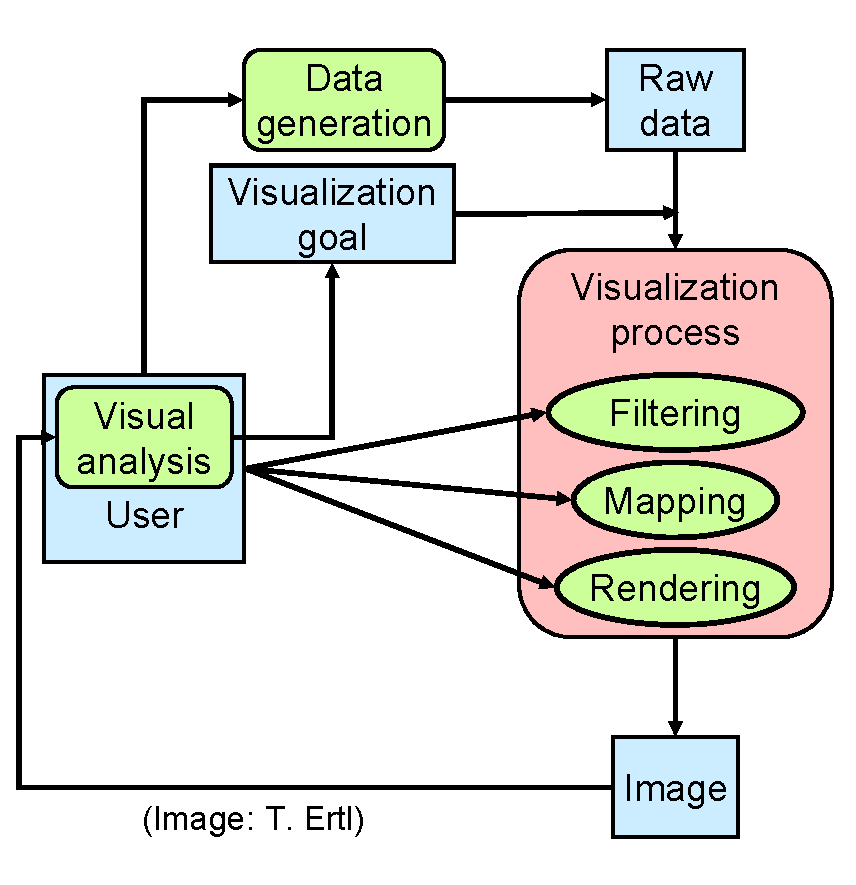
\includegraphics[width=0.5\textwidth]{img/01_vis_scenarios}
\end{figure}
\subsubsection{Video/Movie}
In a first step the data is generated. Then the data is visualised during a batch visualisation step and in the end the video is analized. 
\begin{figure}[H]
    \centering
    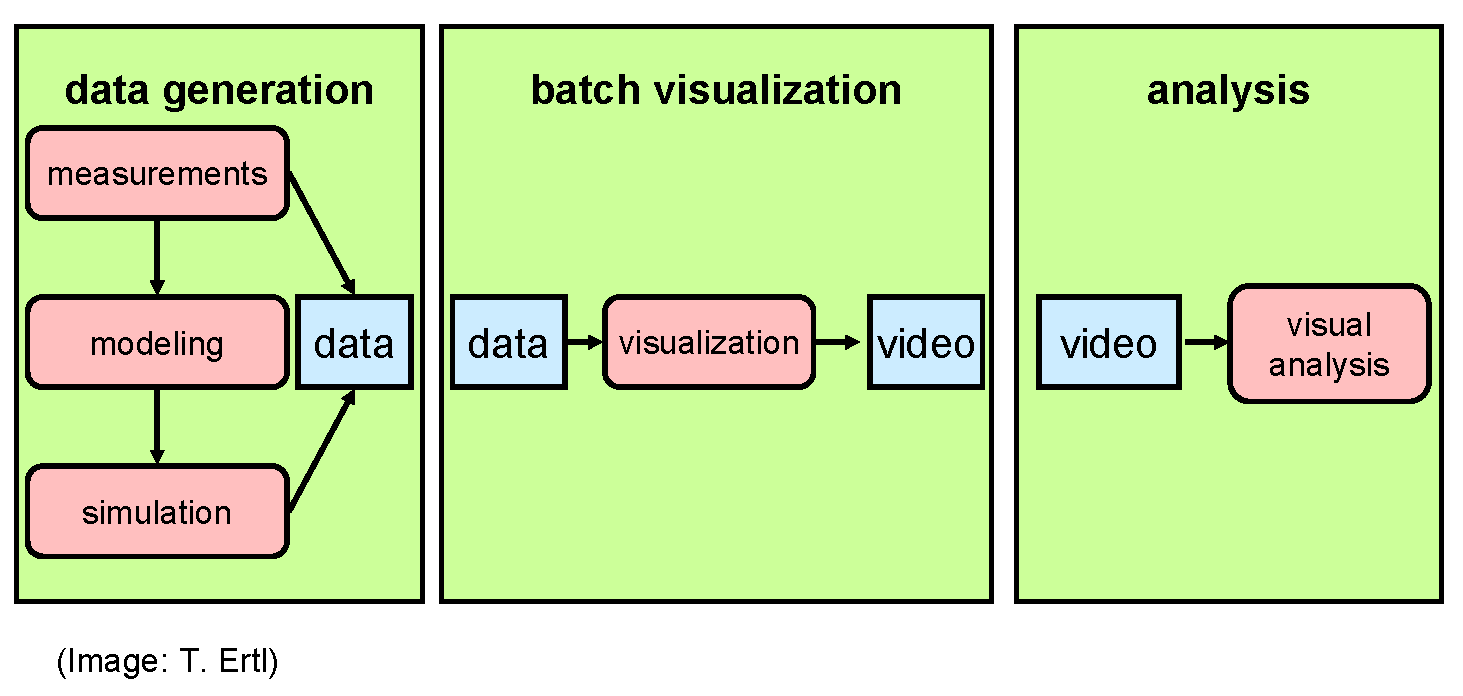
\includegraphics[width=0.75\textwidth]{img/01_movie_mode}
\end{figure}

\subsubsection{Tracking}
The gathered data is directly visualised and analysed.
\begin{figure}[H]
    \centering
    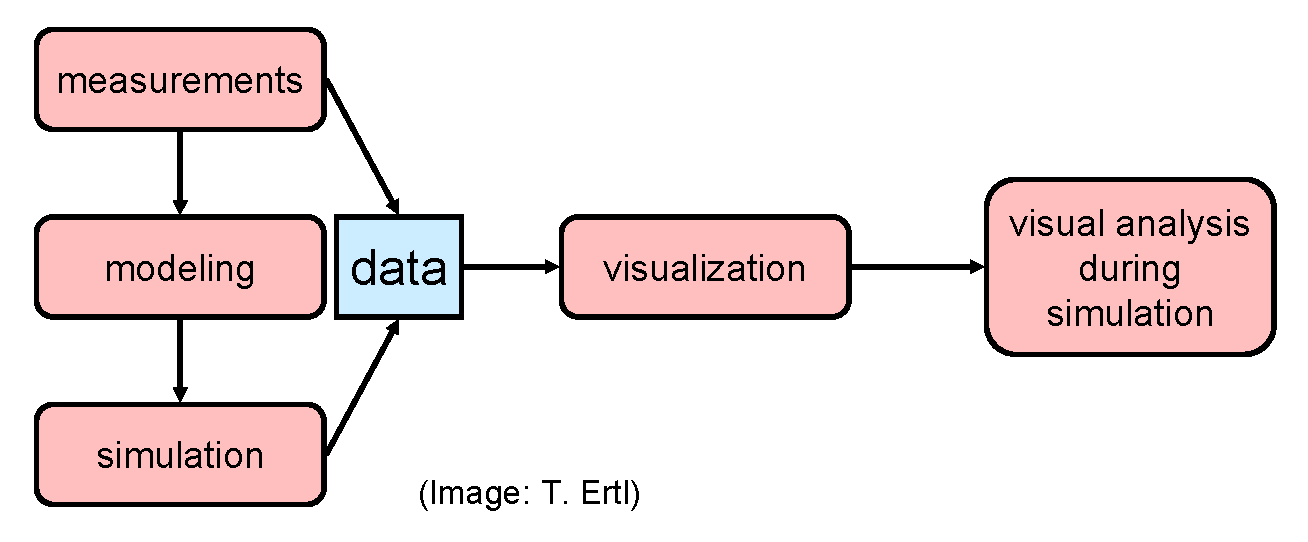
\includegraphics[width=0.75\textwidth]{img/01_tracking}
\end{figure}
\subsubsection{Interactive Post Processing/Visualisation}
The data generation step is split from the visualisation step. 
\begin{figure}[H]
    \centering
    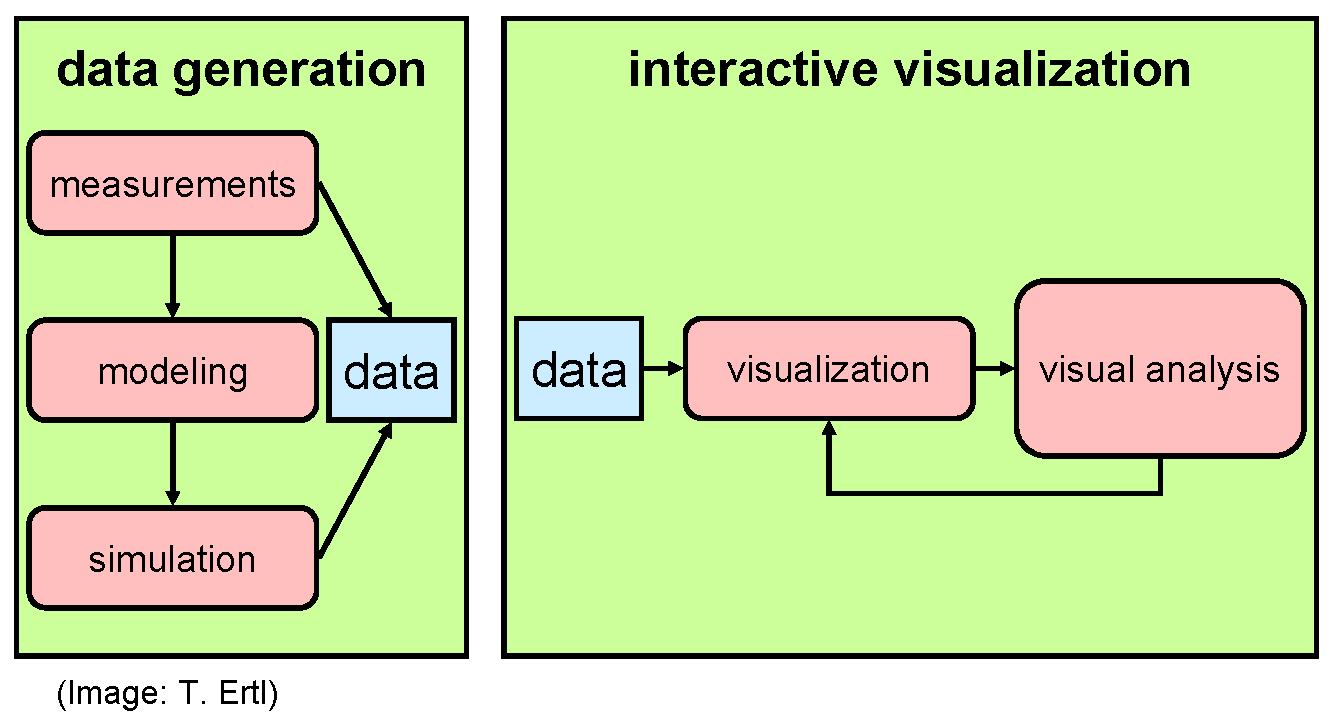
\includegraphics[width=0.75\textwidth]{img/01_interactive_post}
\end{figure}
\subsubsection{Interactive Steering/Computational Steering}
The visualisation has a direct impact on the simulation and the visualisation.
\begin{figure}[H]
    \centering
    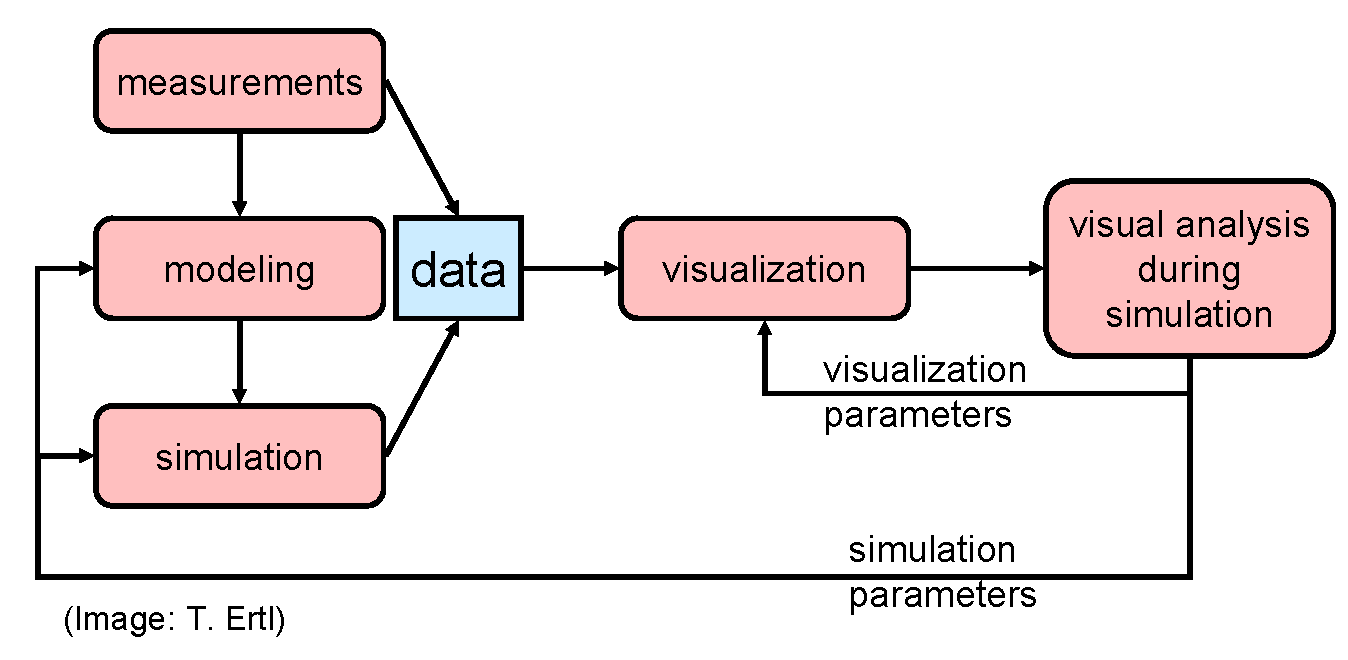
\includegraphics[width=0.75\textwidth]{img/01_interactive_steering}
\end{figure}

\subsection{Data Discretisations}
Types of data sources have typical types of discretisations:
\begin{description}
\item[Measurment Data] Typically scattered ("mesh-less", no grid)
\item[Numerical Simulation Data] $\ $
    \begin{itemize}
        \item Structured, block-structured or unstructured grids
        \item Adaptively refined meshes
        \item Multi-Zone grids with relative motion
        \item ...
    \end{itemize}
\item[Imaging Methods] Uniform grids
\item[Mathematical Functions] (and functionally represented data) can be sampled by demand:
    \begin{itemize}
        \item Uniform
        \item Adaptive
    \end{itemize}
\end{description}

\subsection{Unstructured Grids}
\subsubsection{2D Unstructured Grids}
Cells are \emph{triangles} and/por quadrangles. The domain can be a surface embedded in $3$-space (distinguish $n$-dimensional from $n$-space).
\begin{figure}[H]
\centering   
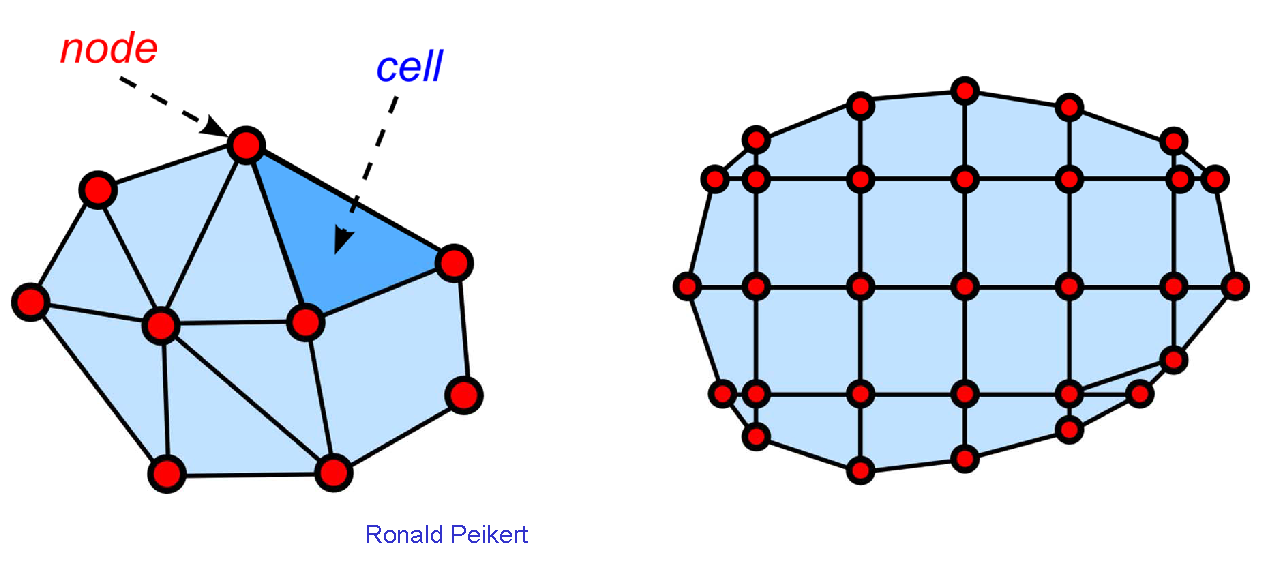
\includegraphics[width=0.75\textwidth]{img/01_unstructured_grids}
\end{figure}

\subsubsection{3D Unstructured Grids}
Cells are \emph{tetrahedra} or \emph{hexahedra}.
\begin{figure}[H]
\centering
\includegraphics[width=0.6\textwidth,page=2]{img/01_3d_unstructured_grids}
\end{figure}
Mixed grids ("zoo meshes") require additional types:
\emph{wedge} ($3$ sided prism), and a \emph{pyramid} ($4$-sided).
\begin{figure}[H]
\centering
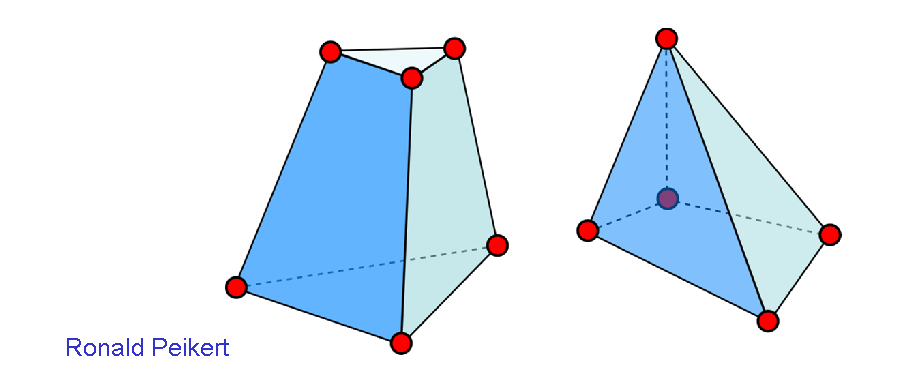
\includegraphics[width=0.6\textwidth,page=1]{img/01_3d_unstructured_grids}
\end{figure}

\subsection{Structured Grids}
\begin{description}
    \item[Curvilinear Grid (general case)] Nodes are given in an array $N_i\times N_j\times N_k$ and the cells are implicit.
    \begin{figure}[H]
        \centering
        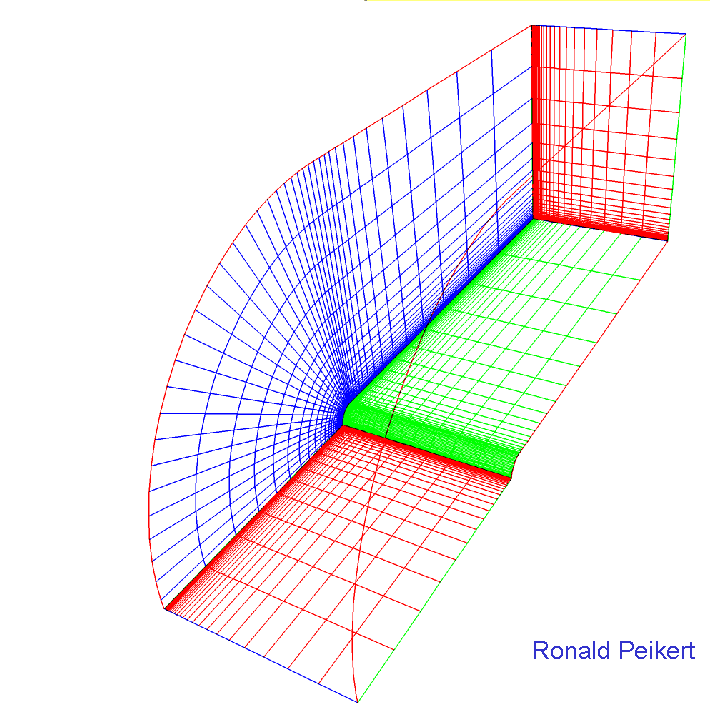
\includegraphics[width=0.5\textwidth]{img/01_curvilinear_grid}
        \caption{Curvilinear Grid}
    \end{figure}

    \item[Rectilinear Grid (special case)] The coordinate functions are simpler:
        \begin{align*}
            x = x(i)\qquad
            y = y(j)\qquad
            z = z(k)
        \end{align*}
        \begin{figure}[H]
            \centering
            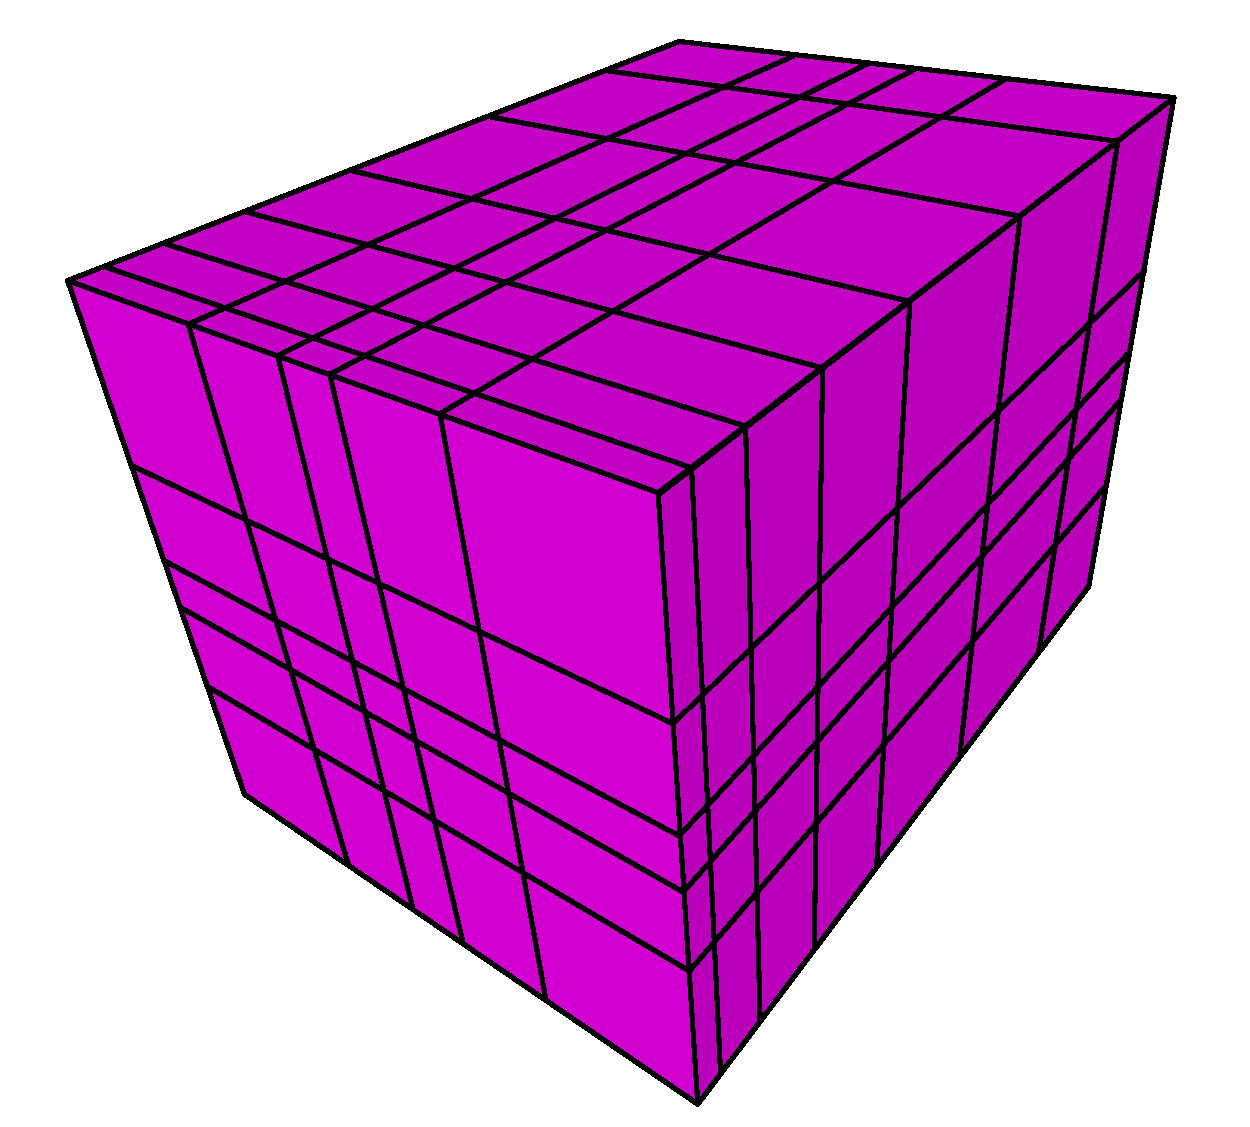
\includegraphics[width=0.25\textwidth]{img/01_rectilinear_grid_wikipedia}
            \caption{Rectilinear Grid, Source: Wikipedia}
        \end{figure}

     \item[Uniform Grid (more special)] The coordinates are defined by an \emph{axis-aligned}bounding box.
\end{description}

\subsubsection{Point-Sampled Data/Scattered Data}
Point sampled data  returns only nodes and no cells. Typical data sources are measurement data for example meteorological data.

Options for visualisation include:
\begin{description}
\item[Point-Based Methods] (relatively few algorithms)
\item[Triangulation] for example constrained Delaunay (difficult in 3D)
\item[Resampling] onto uniform grid.
\end{description}

\subsection{Elementary Visualisation Methods}
\emph{Scalar Fields} can be visualised by plotting its \emph{function graphs}:
\begin{description}
    \item[1D Field:] The Graph is a curve:
        \begin{align*}
            y = f(x)
        \end{align*}
    \item[2D Field:] The Graph is a \emph{height field}:
        \begin{align*}
            z = f(x,y)
        \end{align*}
        Visualisation is easy for rectilinear grids:\\
        \emph{Painter's algorithm} (hidden surface removal in software): Draw cells row by row from back to front.
        \begin{figure}[H]
            \centering
            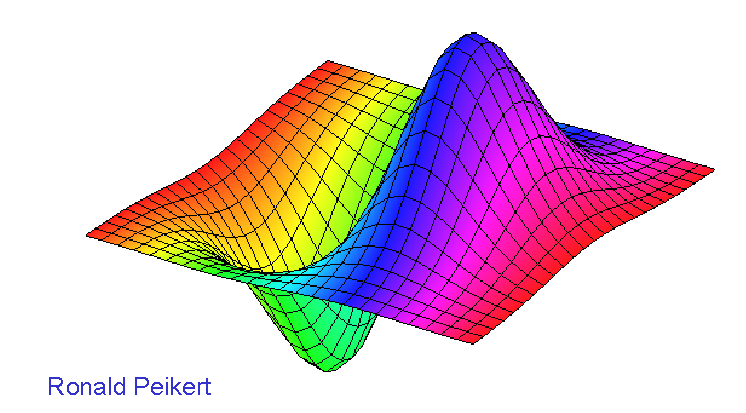
\includegraphics[width=0.7\textwidth]{img/01_painters_algorithm}
        \end{figure}
\end{description}

Scalar fields can also be visualised using \emph{color coding} using \emph{1D texture mapping}. Don't use \emph{vertex colors} and Gouraud shading!
\begin{figure}[H]
    \centering
    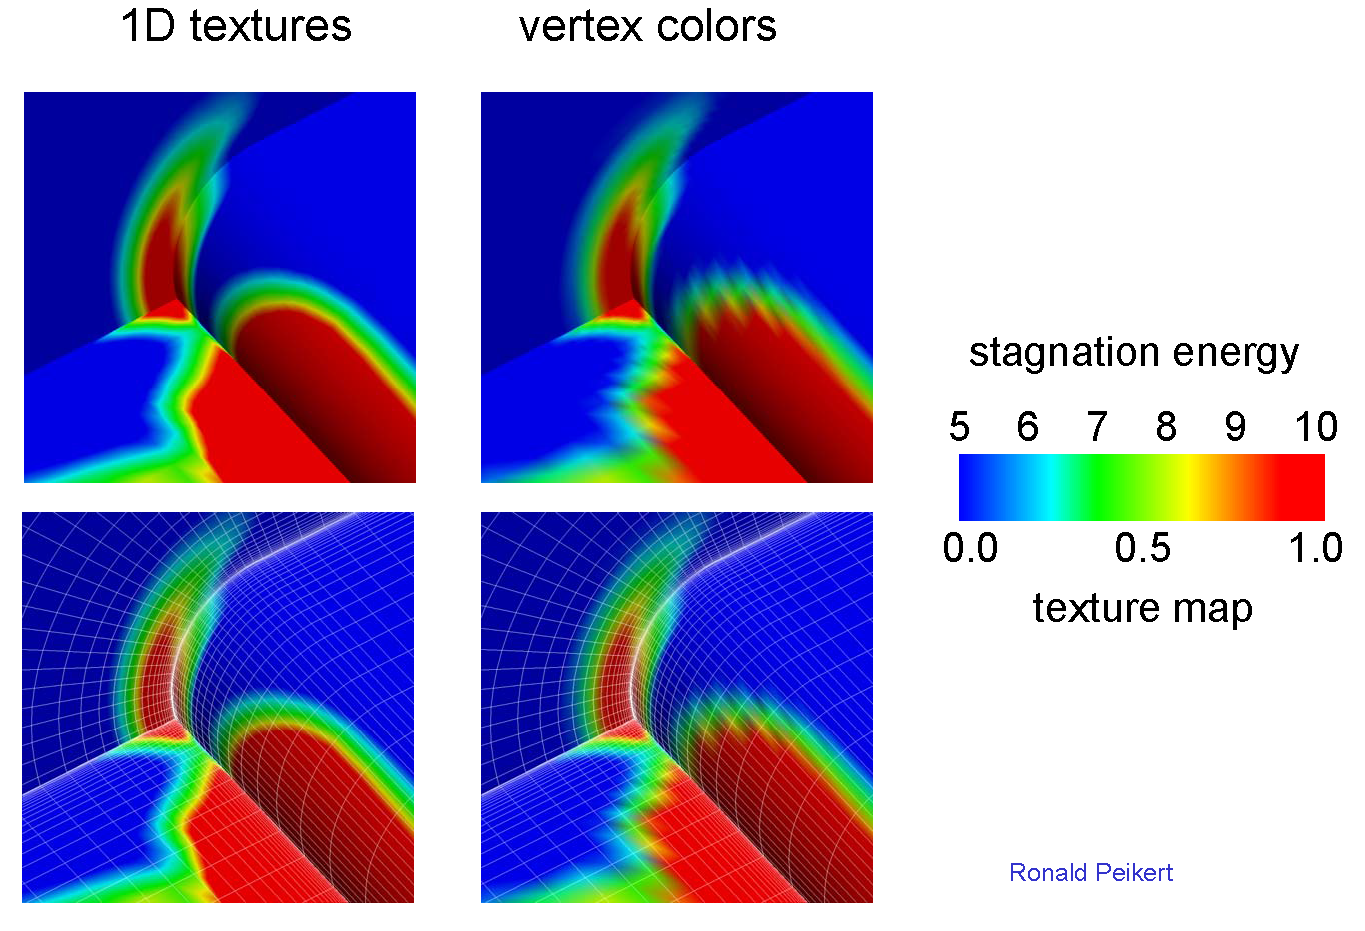
\includegraphics[width=0.9\textwidth]{img/01_texture_mapping}
\end{figure}

\begin{itemize}
    \item Problem of RGB colouring mode: The Interpolation is in the wrong colour space (RGB vs. colour table).
    \item  Problem of Colour Index mode: Lighting is not possible. 
\end{itemize}



\newpage
\section{Contouring and Isosurfaces}

\subsection{Contours}
Contours are a set of points where the scalar field $s$ has a given value $c$:
\begin{align*}
    \left\{ x\in \R^n: s(x) = c\right\}
\end{align*}

Examples in 2D:
\begin{itemize}
    \item Height contours on maps
    \item Isobars on weathermaps
\end{itemize}

\paragraph{Contouring algorithm:}
\begin{itemize}
    \item Find intersection with grid edges
    \item Connect points in each cell
\end{itemize}

\begin{figure}[H]
    \centering
    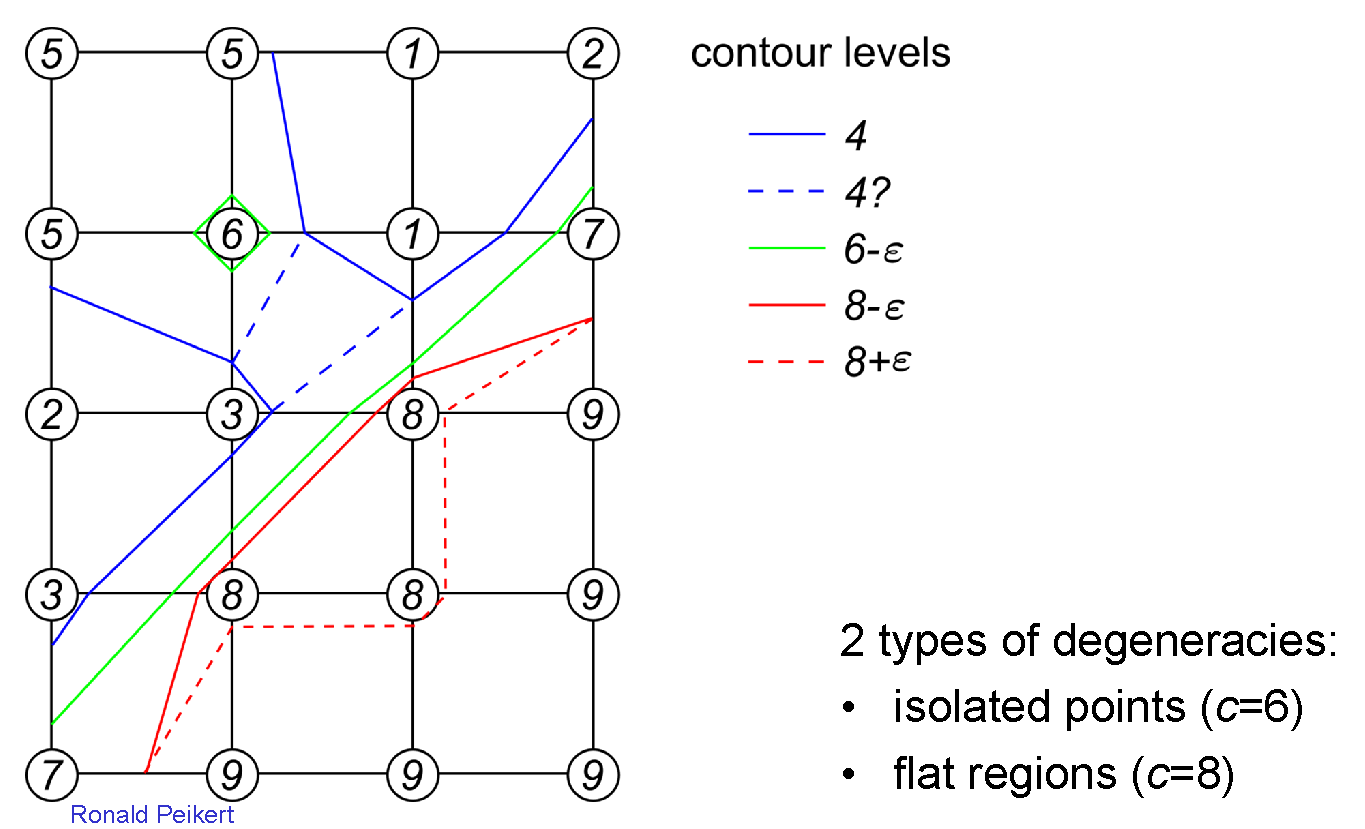
\includegraphics[width=0.75\textwidth]{img/02_contouring_example}
\end{figure}

\paragraph{Topological consistency}
To avoid degeneracies, use \emph{symbolic perturbations}:
\begin{description}
    \item If level $c$ is found as a node value, set the level to $c+\varepsilon$ where $\varepsilon$ is an infinitesimal, i.e., $\varepsilon >0$ and $\varepsilon < x$ $\forall x\in \R$.
\end{description}
Then:
\begin{itemize}
    \item Contours intersect edges at some (possibly infinitesimal) distance from end points.
    \item Flat regions can be visualised by a pair of contours at $c-\varepsilon$ and $c+\varepsilon$.
    \item Contours are \emph{topologically consistent}, meaning:\\
    
        Contours are \emph{closed}, \emph{orientable}, \emph{nonintersecting lines}.    
\end{itemize}

\paragraph{Ambiguities of contours} What is the \emph{correct} contour of $c=4$? 
\begin{figure}[H]
    \centering
    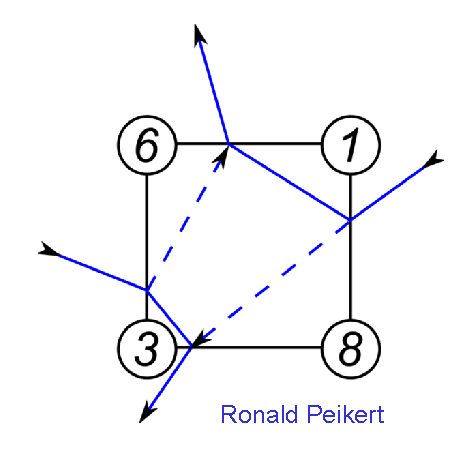
\includegraphics[width=0.3\textwidth]{img/02_contouring_c_4}
\end{figure}
Two possibilities (from which both are orientable):
\begin{itemize}
    \item Connecting the high values \rule{2cm}{0.9pt}
    \item Connecting the low values $- - - - - -$
\end{itemize}

\subsubsection{Contours in a quadrangle cell} 
\begin{description}
\item Local Coordinates $(0,0)\quad (1,0)\quad (0,1)\quad (1,1)$
\item Function Values $\quad s_{00}\quad s_{10}\quad s_{01}\quad s_{11}$
\item Bilinear Interpolant 
    \begin{align*}
     s(x,y) &= (1-x)(1-y)\ s_{00} + x(1-y) \ s_{10}+(1-x)y\ s_{01} + xy\ s_{11}\\
       &= Axy + Bx + Cy + D\\
       \text{with }\quad A &= s_{11}-s_{01}-s_{10}-s_{00}\\
       B &= s_{10}-s_{00}\\
       C &= s_{01}-s_{00}\\
       D &= s_{00}
    \end{align*}
\end{description}

\begin{itemize}
    \item If $A=0$, then the contour equation is $c=Bx+Cy+D$ and the contours are \emph{straight lines}, all parallel.
    \item If $A\neq 0$, then the contour equation is 
        \begin{align*}
            c = A\left( x+{C\over A}\right) (y+{B\over A})+D-{BC\over A}
        \end{align*}
        and the contours are \emph{hyperbola} except for the level
        \begin{align*}
            c = D- {BC\over A}.
        \end{align*}
        
        
        For the special level the contour equation is
            \begin{align*}
                0 = A\left( x+{C\over A}\right) \left( y+{B\over A}\right),
            \end{align*}
        and the contour is a pair of axis-aligned straight lines with
        \begin{align*}
            x &= -{C\over A},\\
            y &= -{B\over A}.
        \end{align*}
\end{itemize}

Decision can be made without computing special level or saddle points by just comparing fractions of edges:
\begin{figure}[H]
    \centering
    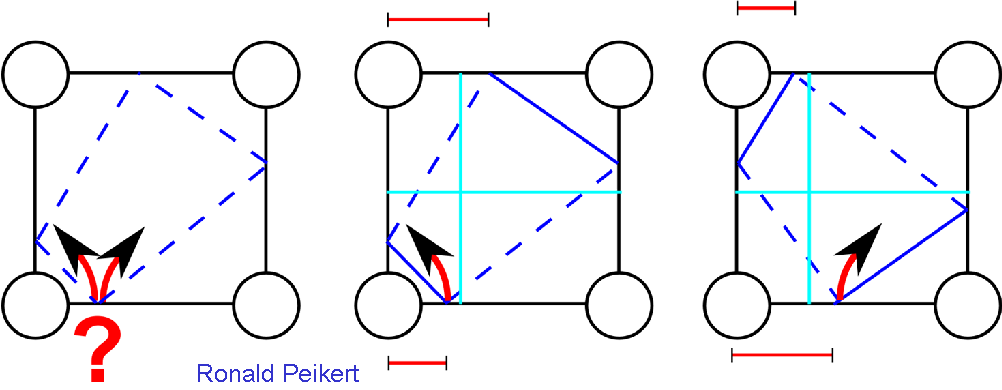
\includegraphics[width=0.75\textwidth]{img/02_contouring_decision}
\end{figure}
By using local coordinates, this works also for curvilinear and unstructured grids.

Not that drawing hyperbola instead of straight lines does not lead to better contours: The piecewise bilinear function is not in $C^1$.

\subsubsection{Basic contouring algorithms}
\begin{description}
    \item[Cell-By-Cell algorithms:] Simple structure, but generate disconnected segments and require post-processing.
    \item[Contour Propagation methods:] Complicated, but generate connected contours.
    \item[Marching Squares algorithm:] Systematic cell-by-cell algorithm. (See below)
\end{description}

\subsubsection{Marching Squares}
Process nodes in ccw (counter-clockwise order), denoted here as $x_0$, $x_1$, $x_2$ and $x_3$. At each node $x_i$ compute the reduced field
\begin{align*}
    \tilde s (x_i) &= s(x_i) - (c-\varepsilon) &\text{(which is forced to be nonzero)}.
\end{align*}
Take it's signe as the $i^{th}$ bit of a $4$-bit integer. Use this as an index for the lookup table containing the connectivity information.
\begin{figure}[H]
    \centering
    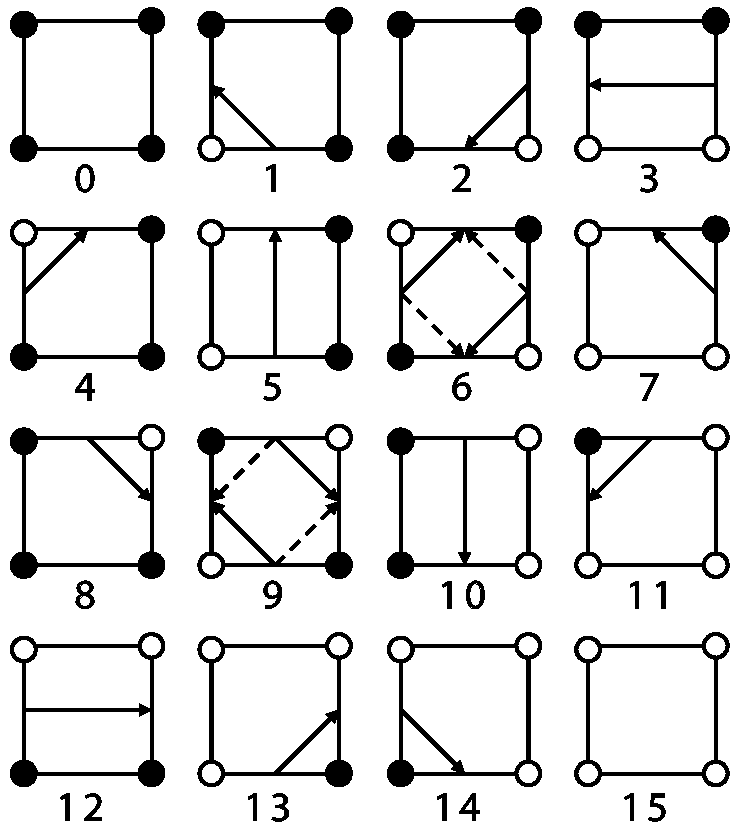
\includegraphics[width=0.5\textwidth]{img/02_marching_squares}
\end{figure}
\begin{align*}
   \bullet\quad \tilde s(x_i) &<0\\
   \circ\quad \tilde s(x_i) &>0
\end{align*}

Alternating signs exist in cases $6$ and $9$. Chose the solid or the dashed line based on topological \emph{consitency}.

\paragraph{Contours in triangle/tetrahedral cells} Linear interpolation of cells implies piece-wise linear contours. Since contours are unambiguous let us introduce a "marching triangles" method. This however introduces periodic artefacts.

\subsection{The Marching Cubes Algorithm}
Contours of $3$D scalar fields are known as \emph{isosurfaces}. Before 1987, isosurfaces were computed as contours on planar \emph{slices}, followed by "contour stitching".

The \emph{marching cubes} algorithm computes contours \emph{directly in 3D}:
\begin{itemize}
    \item Pieces of the isosurfaces are generated on a cell-by-cell basis.
    \item Similar to marching squares, an $8$-bit number is computed from the $8$ signs of $\tilde s(x_i)$ on the corners of a hexahedral cell.
    \item The isosurface piece is looked up in a table with $256$ entries.
\end{itemize}

How to build up the table of $256$ cases?

Lorensen and Cline (1987) exploited $3$ types of symmetries:
\begin{itemize}
    \item Rotational symmetries of the cube
    \item Reflective symmetries of the cube
    \item Sign changes of $\tilde s(x)$.
\end{itemize}

They published a reduced set of $14$ cases:
\begin{itemize}
    \item White circle indicate positive signs of $\tilde s(x)$ ,
    \item The positive side of the isosurface is drawn in red, the negative side in blue.
\end{itemize}

\begin{figure}[H]
    \centering
    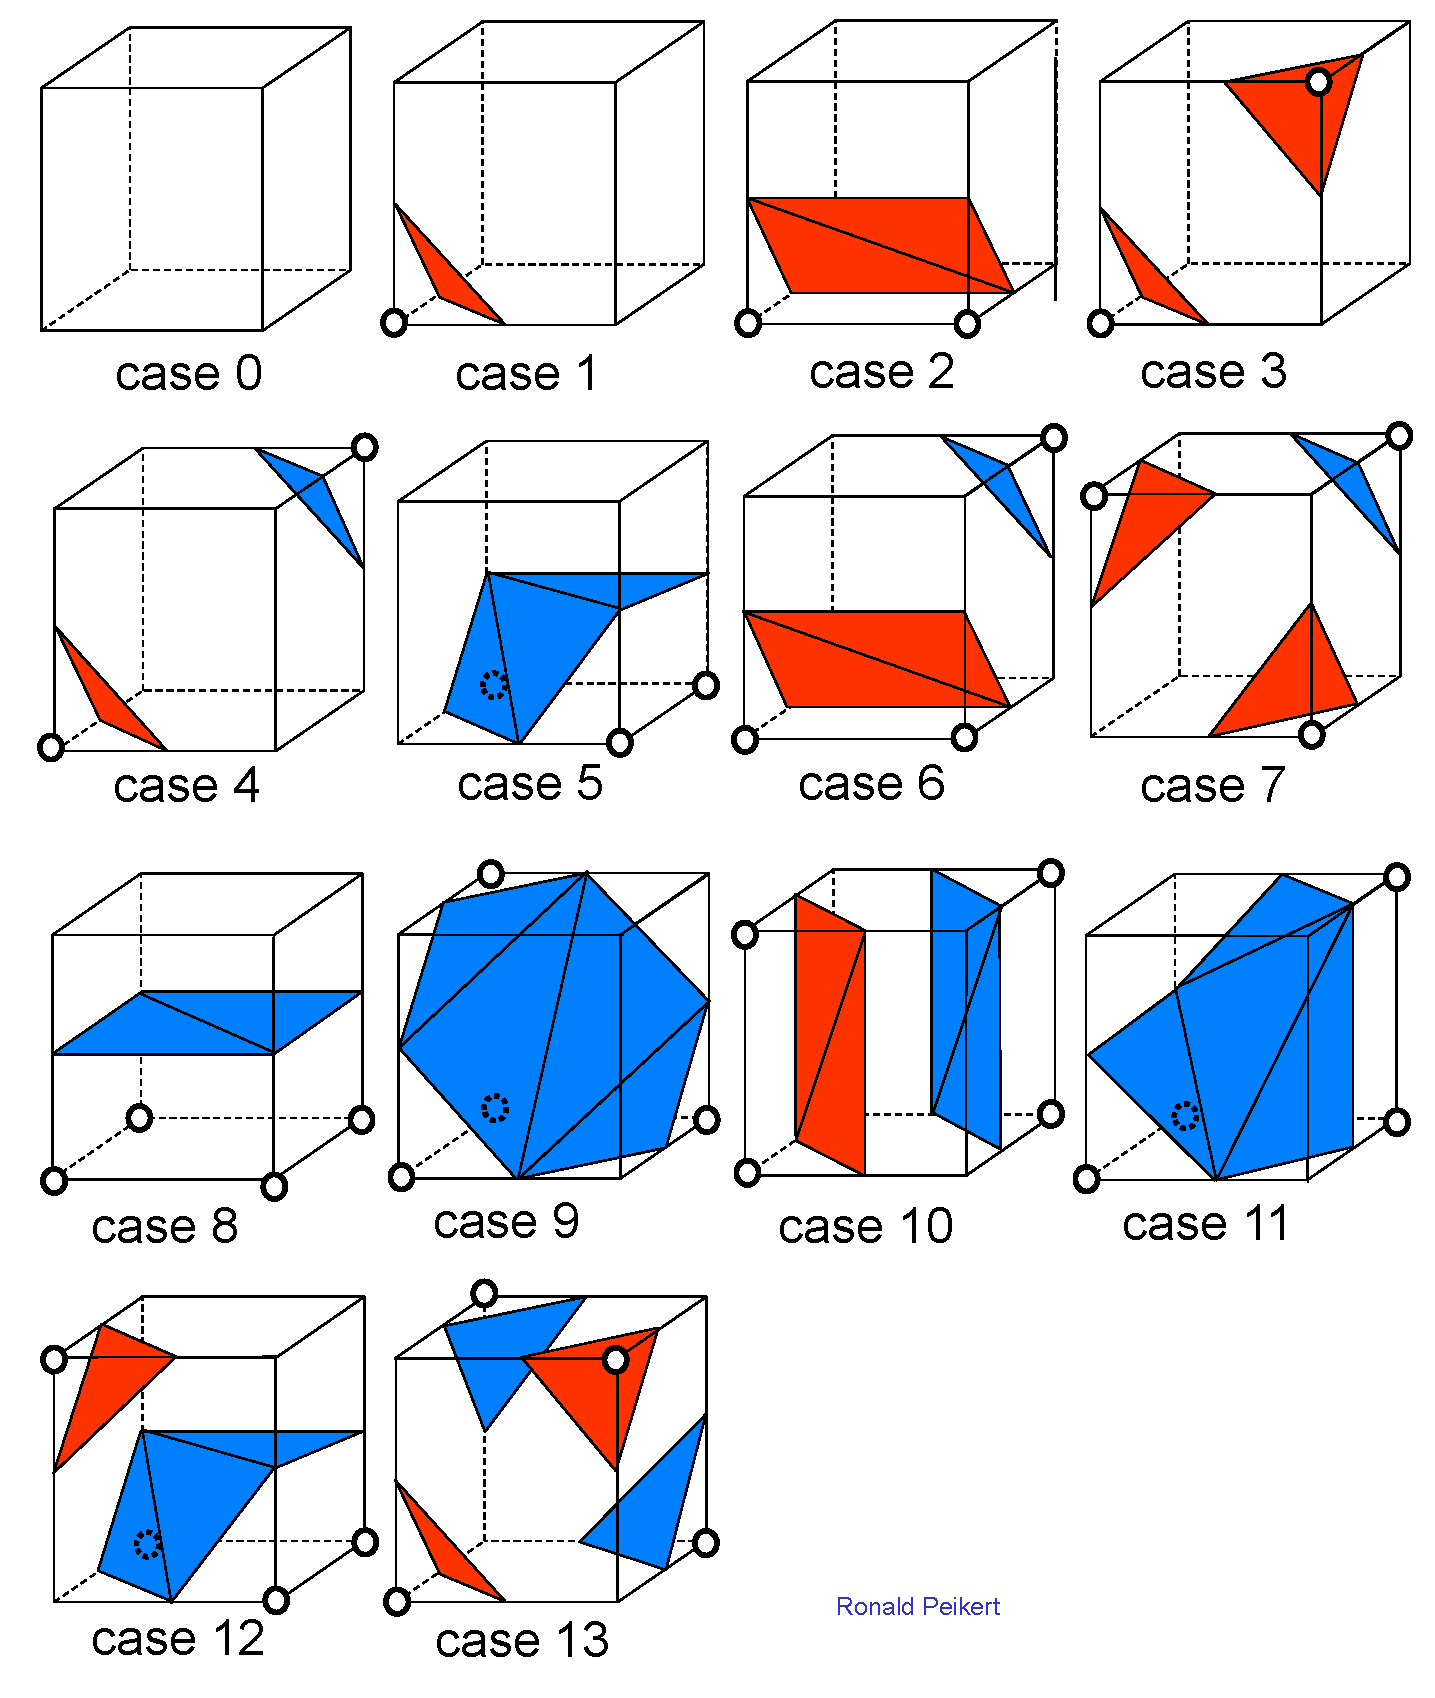
\includegraphics[width=0.75\textwidth]{img/02_marching_cubes}
\end{figure}

Unfortunately not all pieces fit together (same problem as with marching squares) and additional cases need to be introduced. 
\begin{figure}[H]
    \centering
    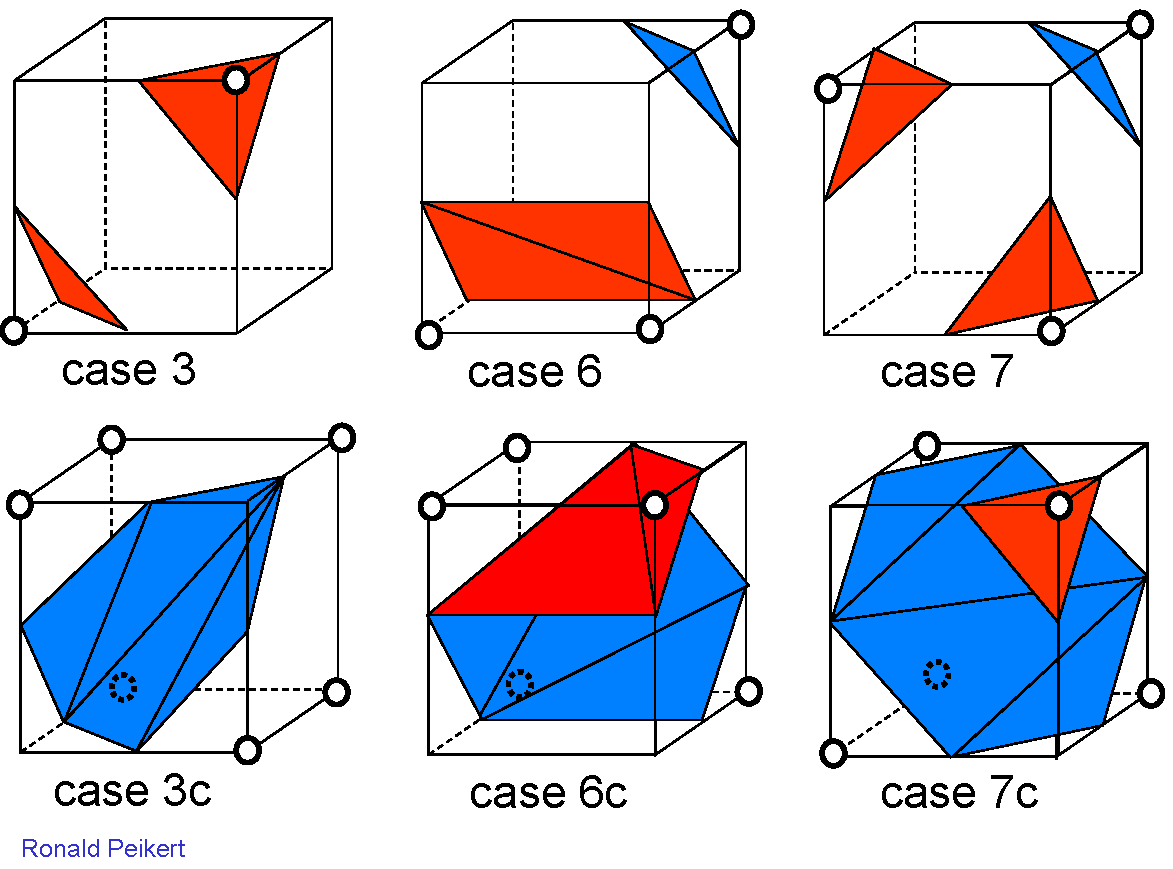
\includegraphics[width=0.75\textwidth]{img/02_marching_cubes_additional_cases}
\end{figure}

The remaining complementary cases are simply obtained by changing the the orientation. Based on these $28$ cases, the full $256$ cases are obtained by rotations of the cube.

\paragraph{Summary} of the algorithm:
\begin{enumerate}
    \item Pre-processing:
        \begin{itemize}
            \item Build a table of the $28$ cases.
            \item Derive a table of the $256$ cases, containing info on
            \begin{itemize}
                \item Intersected cell edges
                \item Triangles based on these points
            \end{itemize}
        \end{itemize}
    \item Loop over cells:
        \begin{itemize}
            \item Find sign of $\tilde s(x)$ for the $8$ corner nodes, giving $8$-bit integer.
            \item Use as index into lookup table.
            \item Find intersection points on edges listed in table, use linear interpolation.
            \item Generated triangles according to table.
        \end{itemize}
    \item Post-processing steps:
        \begin{itemize}
            \item Connect triangles (share vertices)
            \item Compute normal vectors:
                \begin{itemize}
                    \item By averaging triangle normals (problem: thin triangles!).
                    \item By estimating the gradient of the field $s(x)$ (better).
                \end{itemize}
        \end{itemize}
\end{enumerate}

\subsection{The Asymptotic Decider Algorithm}
Motivation for a different isosurface algorithm: Marching cubes can produce "bad" topology.

\emph{Asymptotic decider} algorithm (Nielson and Hamann 1991):
\begin{itemize}
    \item Generate topologically \emph{correct} contours (as oriented straight line segments) on the cell surfaces.
    \item Connect these around the cell, resulting in one or more polygons.
    \item Triangulate the polygons.
\end{itemize}
In general, the AD algorithm generates better isosurfaces. However,
\begin{itemize}
    \item It cannot be easily implemented with a table like Marching Cubes (too many cases).
    \item It generates polygons with up to $12$ sides (Marching Cubes: up to 7).
    \item The topology is correct with respect to the trilinear interpolant, but the geometry can deviate.
    \item Some polygons cannot be "cleanly" triangulated.
\end{itemize}

\subsection{The Dividing Cubes Algorithm}
An early \emph{point-based} algorithm (Crawford et al. '87): For each cell
\begin{itemize}
    \item Check whether it is intersected by the isosurface:
        \begin{align*}
            \min_{i\in \text{cell}} s_i < c < \max_{i\in \text{cell}} s_i
        \end{align*}
    \item Subdivide the intersected cell into $m\times m\times m$ subcells using trilinear interpolation.
    \item Draw the centers of all intersected subcells.
    \item To light the points estimate the gradient and use it as the normal vector.
\end{itemize}

\subsection{Optimised Isosurface Algorithms}
Approaches to speeding up isosurface computation:
\begin{description}
\item[View Dependent] algorithms:
    \begin{itemize}
        \item Occluded triangles are not computed
        \item GPU-based isosurface computation and redenring
    \end{itemize}
\item[Data Processing] for fast computation of \emph{multiple} isosurfaces (multiple levels), for example for interactive exploration of the data.
    \begin{itemize}
        \item Many methods: Octree, Extrema Graph, Span Space.
        \item Common Goal: Avoid computation in non-intersected cells.
    \end{itemize}
\end{description}

\subsubsection{The Span-Space Algorithm}
Method by Livnat (1996).
\begin{enumerate}
\item Pre-Processing. For each element
    \begin{itemize}
        \item Compute $\min$ and $\max$ ,
        \item Treat $(\min,\max)$ as a point in the \emph{span space} (Euclidean plane).
        \item Store points in boxes, non-empty boxes are stored in a linked list.
    \end{itemize}
\item Computation of the isosurface level $c$:

    Find the intersected cells in the \emph{quadrant} $\min < c$, $\max > c$.
    \begin{figure}[H]
    \centering
        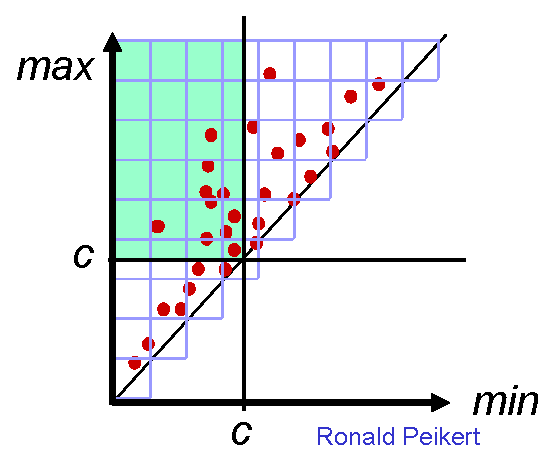
\includegraphics[width=0.5\textwidth]{img/02_span_space_algorithm}    
        \caption{Node distribution in span space.}
    \end{figure}

\end{enumerate}

This algorithm yields a performance gain for datasets with a small local variation, i.e. points in the span space are distributed on the diagonal.

\subsection{Selecting Contour Levels}
Several types of isosurface statistics can help with level selection. 
\begin{figure}[H]
\centering
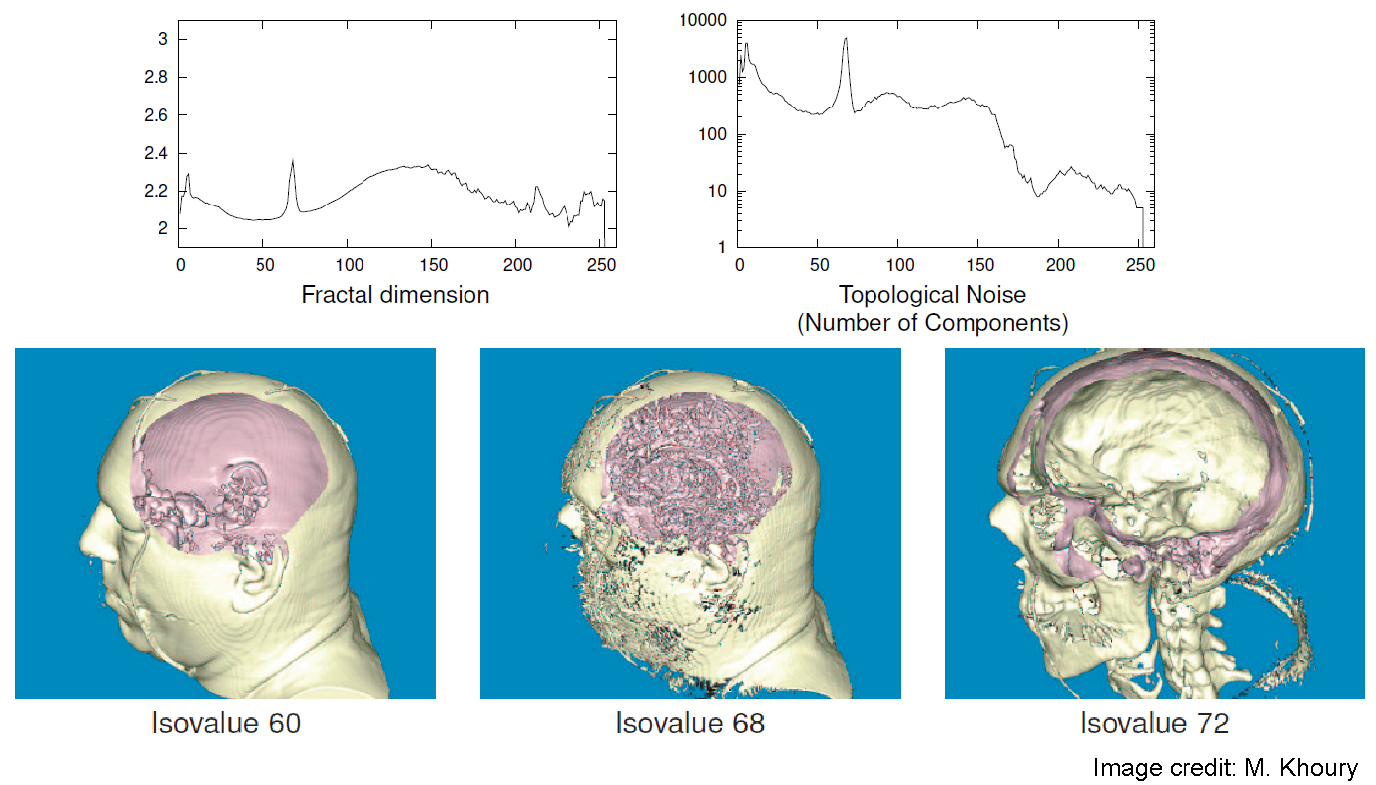
\includegraphics[width=0.9\textwidth]{img/02_contouring_statistics}
\end{figure}

\subsection{Limitations of Isosurfaces}
Isosurfaces represent only a single level within the data range. In practical data, there is often not a single "interesting" level.

Transparent rendering of multiple isosurfaces is possible, but
\begin{itemize}
    \item Limited to a small number of surfaces by visibility
    \item Alpha-blending require depth sorting.
\end{itemize}

Alternatives:
\begin{itemize}
    \item \emph{Feature Extraction methods}, e.g. detecting "blobs" (maximal ellipse-like contours)
    \item \emph{Volume rendering} can show ranges of "interesting levels of the field and/or its gradient.
\end{itemize}








\newpage
\section{Raycasting}

\subsection{Direct Volume Rendering}

Volume rendering (sometimes called \emph{direct volume rendering}) stands for methods that generate images directly from $3$D scalar data. "Directly" means: \emph{no intermediate geometry} (such as an isosurface) is 
generated.

Volume rendering techniques
\begin{itemize}
    \item Depend strongly on the grid type.
    \item Exist for structured and unstructured grids.
    \item Are predominantly applied to uniform grids with $2$D or $3$D image data with \emph{cell-centered} data.
    Cell-centered data 
    \begin{itemize}
        \item are attributed to cells (pixels, voxels) rather than nodes,
        \item can also occur in (finite volume) CFD datasets,
        \item are converted to node data:
            \begin{itemize}
                \item By taking the \emph{dual grid} (easy for uniform grids: $n$ cells $\rightarrow$ $n-1$ cells!),
                \item or by interpolating. 
            \end{itemize}
    \end{itemize}
\end{itemize}


\subsection{Raycasting}
\emph{Raycasting} is historically the first volume rendering technique. It is very similar to \emph{raytracing}:
\begin{itemize}
    \item \emph{image-space} method: The main loop iterates over the pixels of the output image,
    \item a \emph{view ray} per pixel (or per subpixel) is traced backward,
    \item and samples are taken along the ray and \emph{composited} to a single color.
\end{itemize}
The differences are
\begin{itemize}
    \item No secondary (reflected, shadow) rays,
    \item the transmitted ray is not refracted,
    \item more elaborate compositing functions,
    \item and samples are taken at intervals (not at object intersections).
\end{itemize}

\subsubsection{Compositing}
Two simple compositing functions can be used for previewing:
\begin{description}
    \item[Maximum intensity projection] (MIP):
        \begin{itemize}
            \item Maximum of sampled values
            \item Result resembles X-ray image.
        \end{itemize}
    \item[Local maximum Intensity projection] (LMIP):
        \begin{itemize}
            \item Choose first local maximum which is above a prescribed threshold.
            \item Process approximates occlusion.
            \item It is faster and better than MIP.
        \end{itemize}
        \begin{figure}[H]
            \centering
            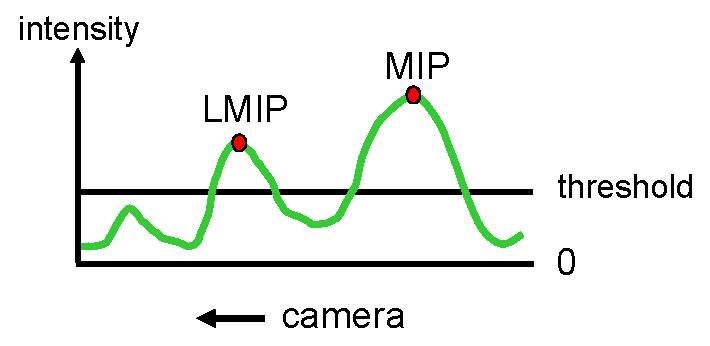
\includegraphics[width=0.6\textwidth]{img/03_lmip}
        \end{figure}
\end{description}

\subsubsection{$\alpha$-compositing}
Assume that each sample on a view ray has a \emph{color} and \emph{opacity}.
\begin{align*}
    (C_0,\alpha_0), \ldots, (C_N,\alpha_N)\qquad\qquad C_i\in [0,1]^3,\ \ \alpha_i\in [0,1]
\end{align*}
where the $0^{th}$ sample is next to the camera and the $N^{th}$ one is a (fully opaque) background sample:
\begin{align*}
    C_N &= (r,g,b)_\text{background}\\
    \alpha_N &= 1.
\end{align*}
$\alpha$-compositing can be defined recursively:

Let $C_f^b$ denot the \emph{composite color} of samples $f$, $f+1$, $\ldots$, $b$. The recursion formula for \emph{back-to-front} compositing yields:
\begin{align*}
    C_b^b &= \alpha_b C_b\\
    C_f^b &= \alpha_f C_f + (1-\alpha_f)C_{f+1}^b.
\end{align*}
With \emph{transparency} set to $T_i = 1-\alpha_i$ we get a \emph{closed formula} for $\alpha$-compositing:
\begin{align*}
    C_f^b = \sum_{i=f}^b \alpha_i C_i \prod_{j=f}^{j-1} T_j
\end{align*}
The \emph{front-to-back} compositing can be derived from the closed formula: Let $T_f^b$ denote the \emph{composite transparency} of samples $f$, $f+1$, $\ldots$, $b$:
\begin{align*}
    T_f^b = \prod_{j=f}^b T_j.
\end{align*}
Then the \emph{simultaneous recursion} for front-to-back composition is:
\begin{align*}
    C_f^f &= \alpha_f C_f\\
    T_f^f &= 1-\alpha_f\\
    C_f^{b+1} &= C_f^b + \alpha_{b+1} C_{b+1} T_f^b\\
    T_f^{b+1} &= (1-\alpha_{b+1})T_f^b.
\end{align*}

\paragraph{The emission-absorption model} How realistic is $\alpha$ compositing? The \emph{emission-absorption} model (Sabella 1988) yields a basic \emph{volume rendering equation}"
\begin{align*}
    L(x) = \int_x^{x_b} \varepsilon (x') \exp\left( -\int_x^{x'} \tau (x'') dx''\right) dx'
\end{align*}
The equation describes the \emph{radiance} arriving along a ray at the position $x$ on this ray. The \emph{emission} function $\varepsilon(x)$ describes the photons "emitted" by the volume along the ray. The \emph{absorbtion} function $\tau(x)$ is the probability that that photon traveling over a unit distance is lost by absorption.


The emission-absorption model is based on the Boltzmann transport equation in statistical physics, but completely \emph{ignores scattering}. In more general models $\tau(x)$ is an \emph{extinction function} having both an absorption term and a scattering term.

Instead, in the emission-absorption model:
\begin{itemize}
\item \emph{Incident scattering} is modelled by the emission function
\item \emph{Loss by scattering} can be thought to be part of the absorption.
\end{itemize}


The discrete version of the emission absorption model:
\begin{align*}
    L(x) = \sum_{i=0}^n \varepsilon_i \Delta x \exp\left( -\sum_{j=0}^{i-1} \tau_j \Delta x \right) 
    = \sum_{i=0}^n \varepsilon_i \Delta x\prod_{j=0}^{i-1} e^{- \tau_j \Delta x},
\end{align*}
matches the $\alpha$-compositing formula
\begin{align*}
    C_f^b = \sum_{i=f}^b \alpha_i C_i \prod_{j=f}^{j-1} (1-\alpha_i)
\end{align*}
and gives interpretations of "opacity" and "color":
\begin{align*}
    \alpha_i &= 1-e^{\tau_j\Delta x} \approx \tau_j \Delta x &\text{if }\Delta x << 1\\
    \alpha_i C_i &= \varepsilon_i \Delta x.
\end{align*}

The product $\tilde C = \alpha_i C_i$ is called a \emph{premultiplied} or \emph{associated} colour.

\subsection{Transfer Functions}
\emph{Transfer functions} map raw voxel data to opacities and colours as needed for the $\alpha$-compositing. Inputs of the TF (one or more):
\begin{itemize}
    \item Voxel value $s(x)$
    \item Gradient magnitude $\norm{\nabla s(x)}$
    \item Higher derivatives of $s(x)$.
\end{itemize}

\begin{description}
\item \emph{Opacity transfer function} $\alpha(s(x), \norm{\nabla s(x)}, \ldots)$
\item \emph{Color transfer function} $C(s(x), \norm{\nabla s(x)}, \ldots)$
\end{description}

In general TF don't depend on \emph{spatial location}, exception for \emph{focus and context} techniques.

By choosing different opacity transfer functions different types of applications can be achieved.
\begin{figure}[H]
\centering
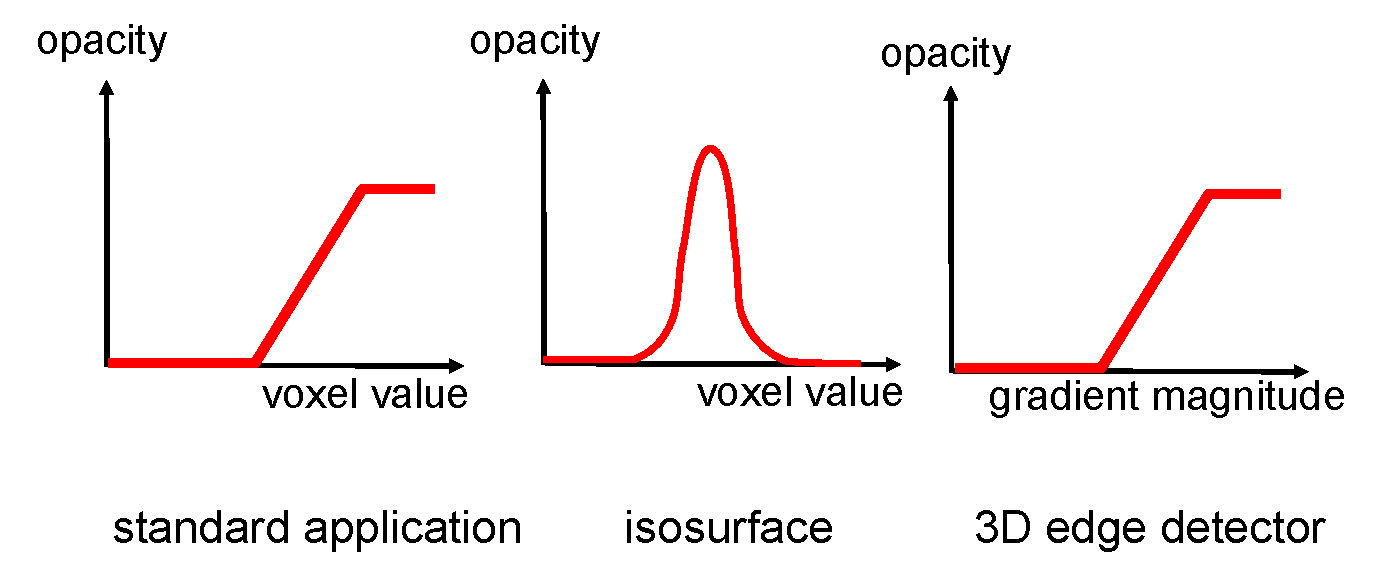
\includegraphics[width=0.8\textwidth]{img/03_tf_types}
\end{figure}

Example of a \emph{bivariate} (=2D) transfer function:
\begin{figure}[H]
    \centering
    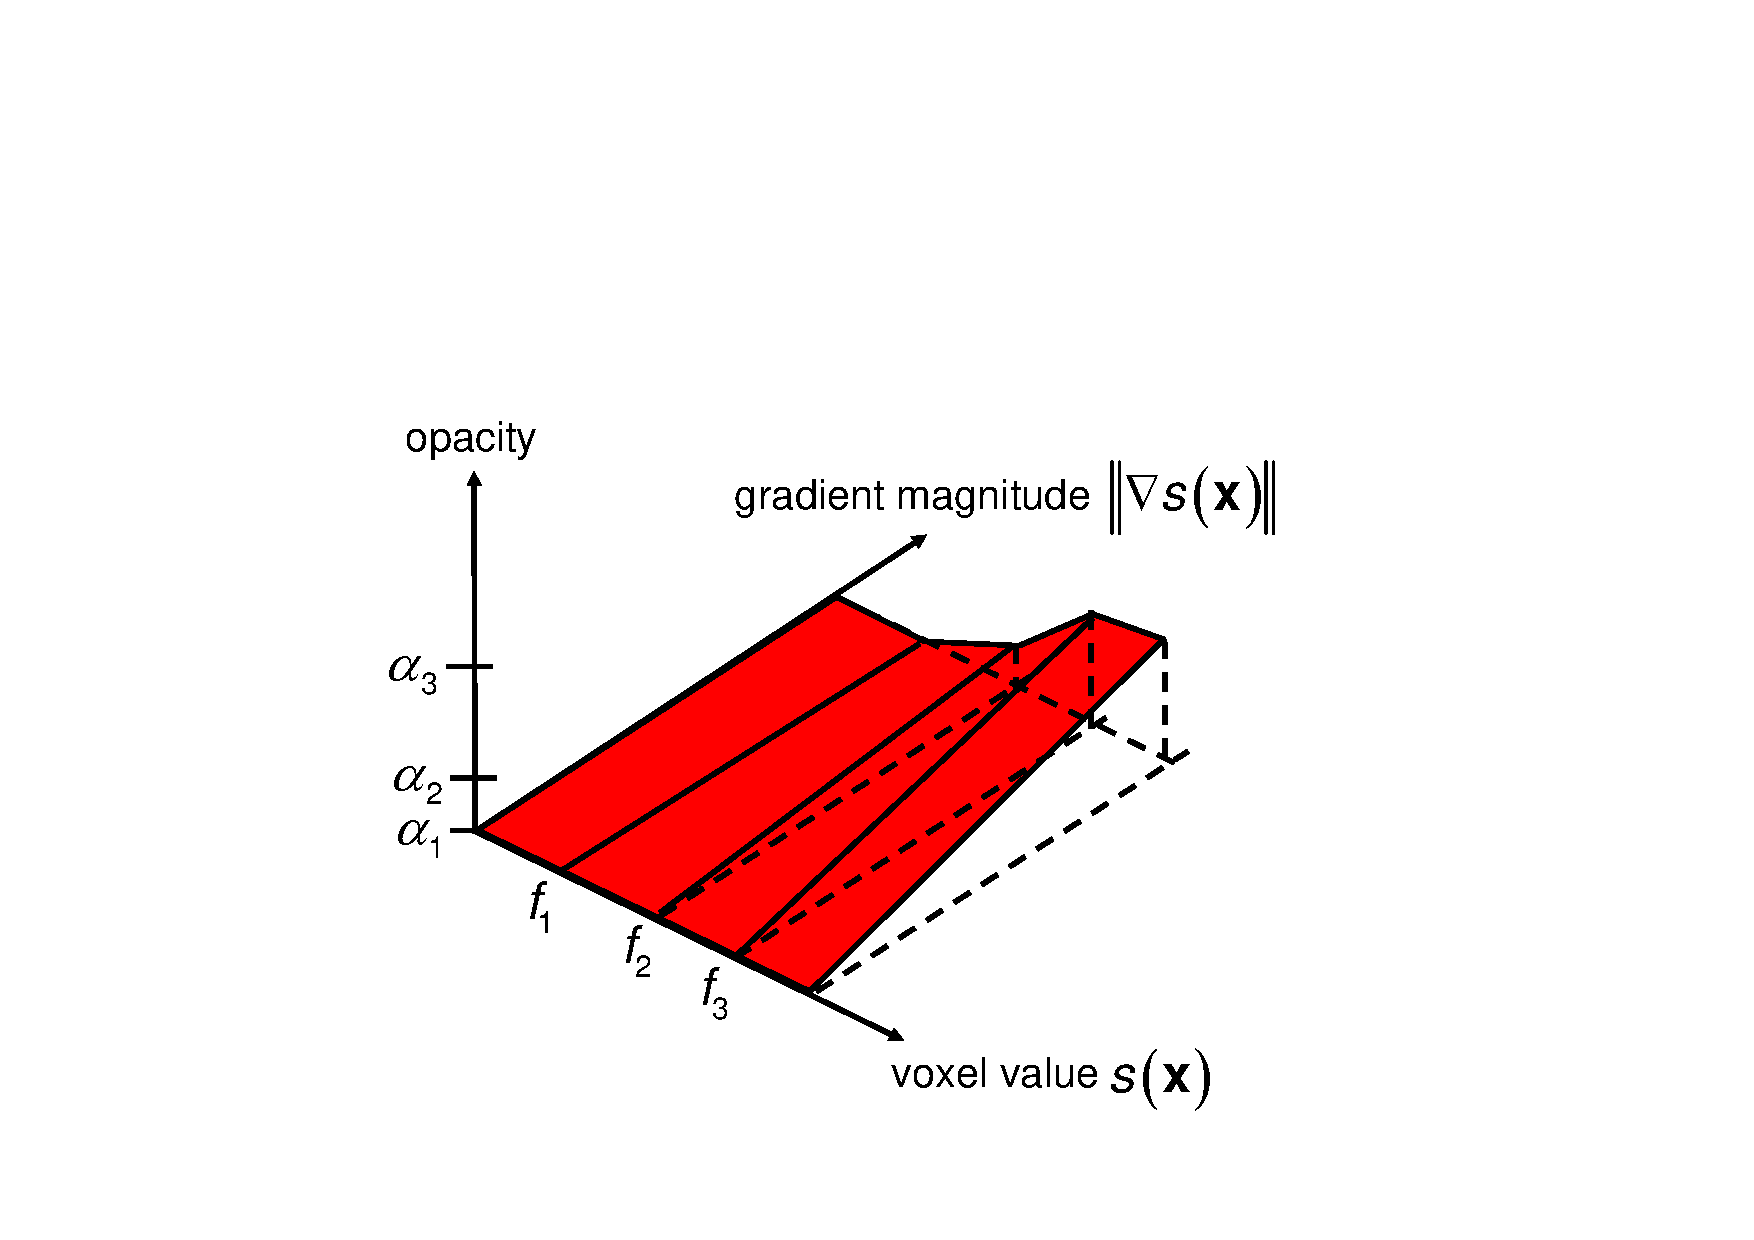
\includegraphics[width=0.6\textwidth,page=1]{img/03_tf_bivariate}
\end{figure}
Example of a bivariate transfer function for an isosurface of constant thickness.
\begin{figure}[H]
    \centering
    \includegraphics[width=0.6\textwidth,page=2]{img/03_tf_bivariate}
\end{figure}

The color transfer function allows to make a simple \emph{classification}.
\begin{figure}[H]
    \centering
    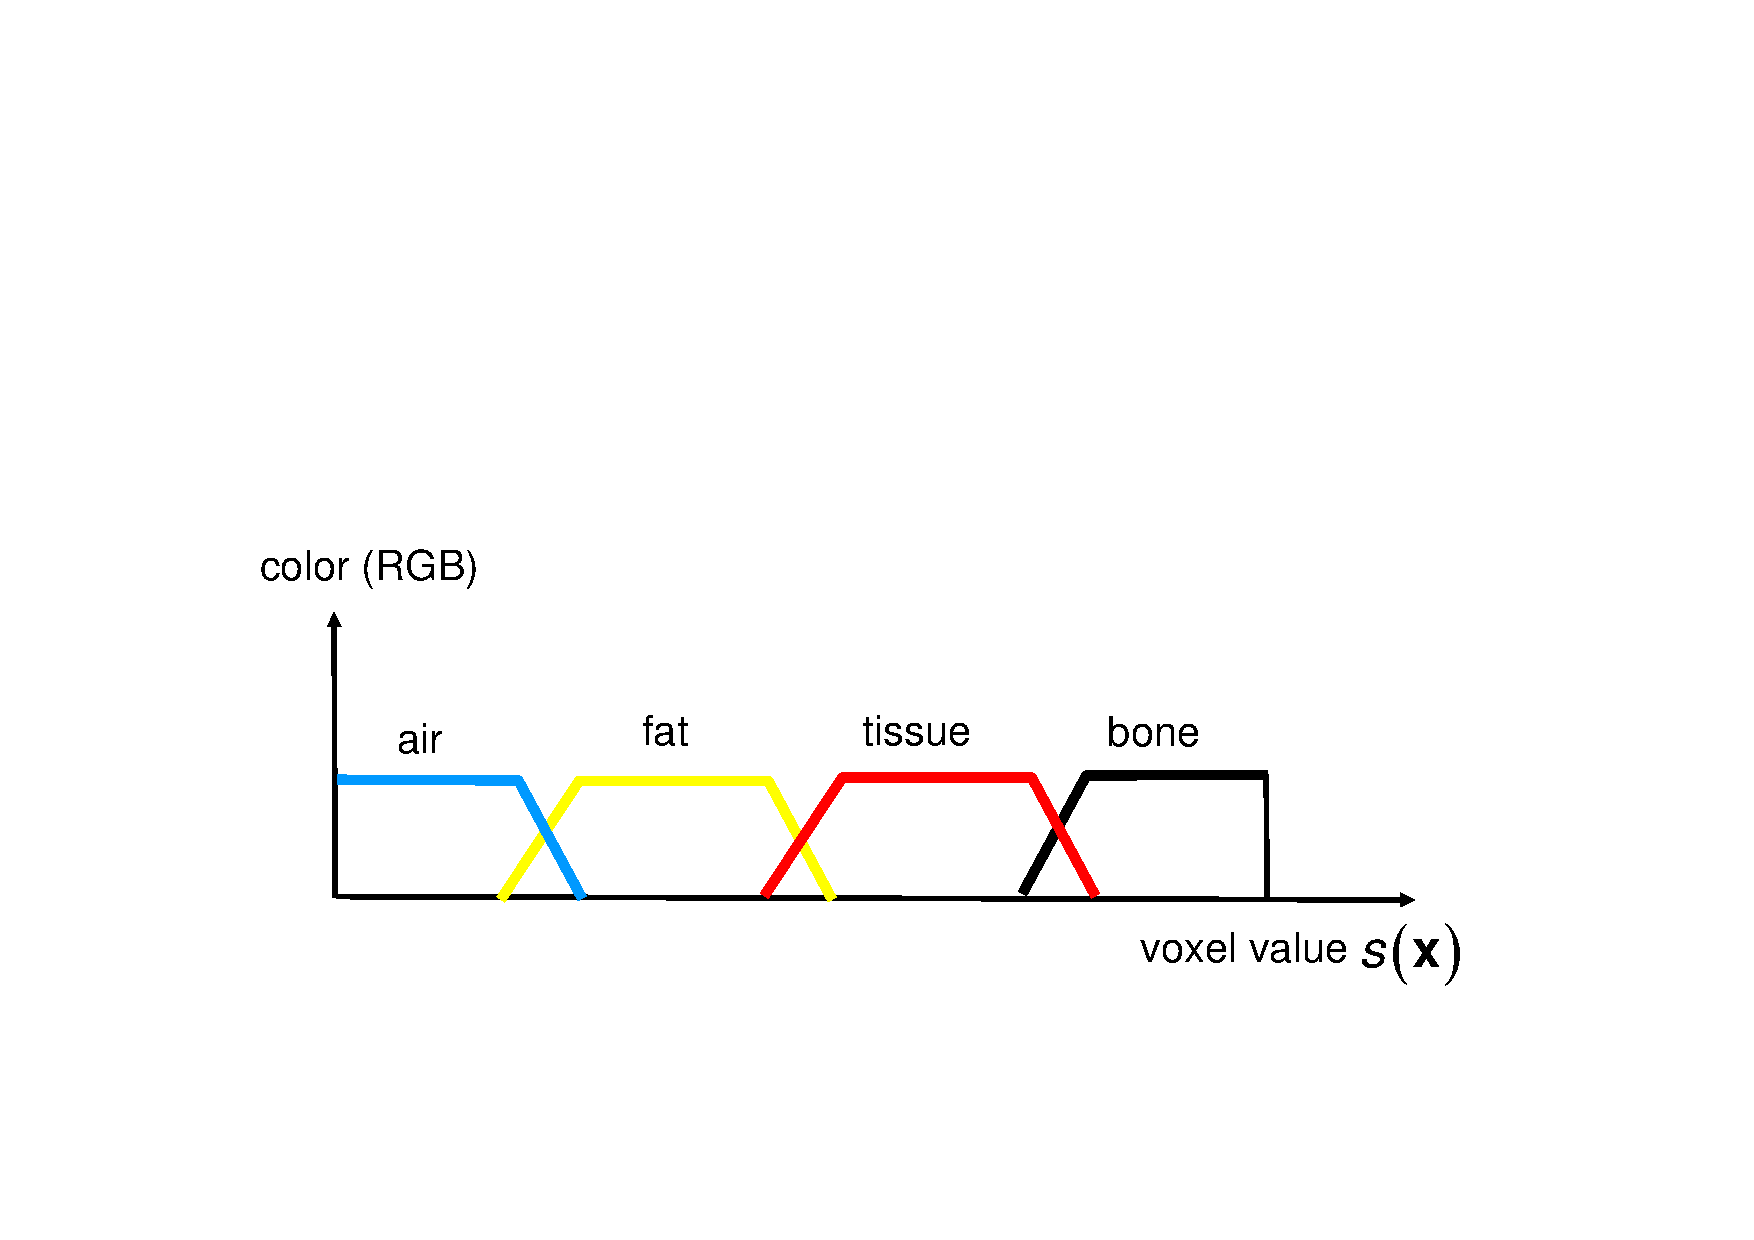
\includegraphics[width=0.8\textwidth,page=1]{img/03_tf_color}
\end{figure}

\paragraph{Pre-classification} In pre-classification, the voxels can also be lit:
\begin{itemize}
    \item The gradient is perpendicular to the local isosurface. It can be used as a normal vector for \emph{Phong lighting} (without rendering the isosurface itself).
    \item \emph{Reflection coefficients} can be assigned by a separate transfer function ("materials" instead of only colors).
    \item \emph{Diffuse lighting} can be applied to the entire volume dataset as a pre-processing since it's independent of the viewing direction.
\end{itemize}

\subsubsection{Pre- vs. Post-classification}
For quality reasons, current volume rendering implementations often use \emph{post-classficiation}.

\begin{description}
\item[Pre-Classification] $\ $
    \begin{enumerate}
        \item Transfer functions are applied to voxels.
        \item Results are interpolated to sample locations.
    \end{enumerate}
\item[Post-Classification] $\ $
    \begin{enumerate}
        \item Raw data are interpolated to sample locations.
        \item Transfer functions are applied to sampled data.
    \end{enumerate}
\end{description}

\subsection{Preintegration}
Idea (Engel 2001): Simulate \emph{infinitely many} interpolated samples between two successive samples $s_i= s(x_i)$ and $s_{i+1} = s(x_{i+1})$. Assuming that 
\begin{itemize}
    \item Field $s(x)$ varies \emph{linearly} between samples
    \item and that the transfer functions don't depend on derivatives.
\end{itemize}

The discrete formula for opacity at a sample was
\begin{align*}
    \alpha_i = 1-e^{-\tau_i \Delta x}.
\end{align*}
The continuous version for a sample interval $[x_i, x_{i+1}]$ is 
\begin{align*}
    \alpha_i = 1-e^{-\int_{x_i}^{x_{i+1}} \tau(s(x)) dx}.
\end{align*}
Assuming now $s(x)$ to be linear between samples, we get:
\begin{align*}
    \alpha_i &= 1-\exp\left( {-{d\over s_{i+1}-s_i} \int_{s_i}^{s_{i+1}}\tau(s) ds}\right) &\text{with } d= \norm{x_{i+1}-x_i}, 
\end{align*}
which is called a \emph{preintegrated opacity transfer function}.


The integral
\begin{align*}
\int_{s_i}^{s_{i+1}} \tau(s) ds = \int_0^{s_{i+1}} \tau(s) ds - \int_0^{s_i} \tau(s)ds
\end{align*}
can be evaluated by two lookups in a precomputed table of 
\begin{align*}
\int_0^{s} \tau(s')ds'.
\end{align*}

The composite colour of the same interval
\begin{align*}
  C_i = \int_{x_i}^{x_{i+1}} \varepsilon (s(x))\exp\left(-\int_{x_i}^x \tau(s(x'))dx'\right) dx,
\end{align*}
simplifies for linear $s(x)$ to:
\begin{align*}
  C_i = {d\over {s_{i+1}-s_i}} \int_{s_i}^{s_{i+1}} \varepsilon (s)\exp\left(-{d\over {s_{i+1}-s_i}} \int_{s_i}^x \tau(s')ds'\right) ds,
\end{align*}
which can be precomputed for all combinations of $s_i$, $s_{i+1}$ and $d$.

\subsubsection{Extinction-based volume rendering}
Instead of an opacity Transfer function, use an extinction TF [Schlegel 2011]. Advantage: Extinction is \emph{additive}.
\begin{itemize}
    \item Riemann sums for numerical integration give better accuracy.
    \item Additivity can be used for efficient lighting.
\end{itemize}

\paragraph{Screen-Space ambient occlusion} Approximate the fraction of ambient light that is occluded. Method: Compute the total extinction per shell (boxes approximating spheres) b using a \emph{summed area table}.




\end{document}
